\documentclass[12pt, fleqn]{article}

\usepackage{amsfonts,amsthm,amsopn,amssymb,latexsym}
\usepackage{graphicx}
\usepackage[pdftex]{hyperref}
\usepackage[T1]{fontenc}
\usepackage[brazil]{babel}
\usepackage[utf8]{inputenc}
\usepackage{a4wide}
\usepackage[intlimits]{amsmath}
\usepackage{multirow}
\usepackage{placeins}               
\usepackage{url}
% \usepackage{indentfirst}

% \setlength{\parindent}{6pt}
\setlength{\textwidth}{16.0cm}        % largura do texto
\setlength{\textheight}{9.0in}        % tamanho do texto (sem head, etc)
\renewcommand{\baselinestretch}{1.15} % espa�amento entre linhas
\addtolength{\topmargin}{-1cm}        % espa�o entre o head e a margem
\setlength{\oddsidemargin}{-0.1cm}    % espa�o entre o texto e a margem

% Ser indulgente no preenchimento das linhas
\sloppy 

\begin{document}

    \pagestyle {empty}

    \vspace*{-2cm}
{\bf
\begin{center}
  {\large
  \hspace*{0cm}Universidade Federal de Juiz de Fora} \\
  \hspace*{0cm}Departamento de Ciência da Computação \\
  \hspace*{0cm}DCC059 - Teoria dos Grafos Semestre 2015-2  \\
\end{center}}
\vspace{4.0cm}
% \noindent
\begin{center}
  {\Large \bf Problema de cobertura de vértices ponderados com minimização de vértices } \\[4cm]
  {\Large Daniel André Carlos Cândido}\\[6mm]
  {\Large Professor: Stênio Sã Rosário F. Soares}\\[3.0cm]
\end{center}

{\raggedleft
\begin{minipage}[t]{8.3cm}
  \setlength{\baselineskip}{0.25in}
  Relatório da terceira parte do  trabalho de Teroria dos Grafos, parte integrante da avaliação da disciplina.
\end{minipage}\\[1cm]}

\vspace{4cm}
{\center Juiz de Fora \\[1mm]
Março de 2016 \\}

\newpage
    
    
    \pagestyle {empty}
    
    \newpage

    \pagestyle {plain}

    \setcounter{page}{0} \pagenumbering{arabic}
    
    \setlength{\parindent}{0in}  
    
    \parskip 5pt  

    \section{Introdução}

    %comando cria itens
      \quad Em Teoria dos Grafos, cobertura de vértices de um grafo trata-se de um conjunto de vértice tal que cada aresta do grafo é incidente, a pelo menos, 
	   um vértices do conjunto, ou seja, é um conjunto de vértices que contém pelo menos uma das extremidades de cada aresta. 
	   Em outras palavras, uma cobertura de vértices é um conjunto V de vértices que obedece a seguinte propriedade: toda aresta do grafo tem pelo menos uma das extremidades em um vértice de V.
      
      \quad Cobertura de vértices ponderado com minimização de vértices, concite em encontra um número mínimo de vértices que possua o menor peso possível e que  atenda a propriedade citada acima.      
      
      \quad Uma aplicação prática para o problema é definir a melhor localização “possível” para uma instalação de antena de celular ou uma minimização do número de instalações de câmera de segurança.


    \section{Metodologia utilizada}
      \quad Dentre as linguaguens de programação propostas, C++ foi a linguagem escolhida para implementar deste trabalho. 
	Pois, trata-se de uma abordagem flexível e multiparadigma permitindo ainda o uso de orientação a objetos, programação genérica e em alguns casos o uso de ambos em um mesmo código. 
	Uma outra vantagem está nos problemas relacionados à memória, visto que nesses casos é possível adotar um estilo de mais baixo nível.


      \subsection{Estruturas de dados utilizadas}	
	\quad O algoritmo implementado possui as seguintes classes: 
	
	  \begin{itemize}
	      \item Classe Grafo: Responsável pelas manipulações do grafo em si. 
	      O grafo é representado por listas de adjacências, e para cada vértice há uma lista encadeada contendo suas arestas com os demais vértices do grafo. 
	      As listas são compostas de item e são representações de grafos, logo grafos são listas, e essa relação pode portanto, ser definida como herança simples. 
	      Os vértices estão definidos como listas de arestas e itens do grafo, ou seja herança múltipla. As arestas, por sua vez, são apenas itens dos vértices o que nos faz apresentar outro exemplo de herança simples. 
	      
	      \item Classe Vértice: Utilizada para manipulações referentes às arestas. Suas funções se referem basicamente a: verificar existência de arestas,
	      encontrar arestas, e remover arestas (ambas apresentando o valor do id do vértice como parâmetro).
	      
	      \item Classe Item: Possui operações referentes à lista encadeada. Como por exemplo, pegar próximo, pegar anterior, pegar informação, entre outras.
	      
	      \item Classe Lista: Apresenta as operações referentes à lista de vértices. Como por exemplo, contar número total de itens, adicionar e deletar item, entre outras.
	      
	      \item Classe LeituraGravacao: Responsável pela leitura e gravação dos arquivos de texto. Sendo que os arquivos de leitura são as instâncias contendo os grafos. 
	  \end{itemize}


      \subsection{Abordagens utilizadas}
	\quad Foram adotadas três abordagem na elaboração do trabalho,  Construtivo (Guloso), Construtivo Randômico e Construtivo Randômico Reativo ou Adaptativa.
	
	  \begin{itemize}
	    \item Algoritmo Construtivo:
		\par Concite em escolher sempre o melhor candidato de uma lista de canditato previamente ordenada.
	      \begin{figure}[!htpb]
% 		\centering
		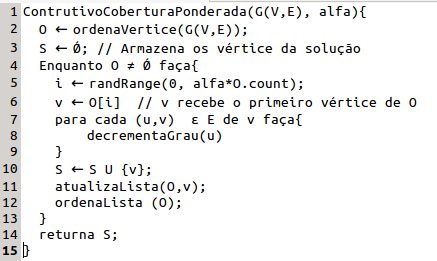
\includegraphics[scale=0.8]{contrutivo.png}
% 		\caption{Algoritmo Flody-Warshall, a primeira matriz sem a execução do algoritmo, a segunda e resuldado do algoritmo e a terceira represeta o menor caminho do vértice v para cada vértice u}
		\label{fig:contrutivo}
	      \end{figure}  
	      
	      \par O algoritmo construtivo, recebe como parametro o grafo e um alfa que no caso cdo guloso esse valor é zero, 
	      para que o algoritomo comece do inicio do array. Na linha 2, na imagem acima, é criado um lista de candidatos ordenado pela divisão  P $\div$ g, onde P é o peso e g o grau do vértice, na linha 3 é criado um conjunto vazio.
	      A condição de para do algoritmo é quando um array ciaro na linha 2 está vazio.	      
	      \par Nas lihas 5 e 6, o indece i sempre recebe zero (nesse caso por conta do valor de alfa ser igual a zero)
		    e o vetor v recebe o primeiro elemnte da lista O(lista de candidatos).	
	      \par Entre as linha 7 a 9, o grau dos vértice adjacência a v é decrementato em uma unidade. 
		    Nas linhas de 10 a 14, a lista de solução recebe o vértice v,
		    a lista de cadidatos O é atualizada e a por fim é retornado a soução na linha 14. 
	    
	    \newpage
	    
	    \item Algoritmo Contrutivo Randômico:
		\par Concite em escolher o melhor canditato entre os x melhores candidatos de uma lista L de canditato previamente ordenada. 
		Onde o tamnha de x é dado pelo tamanha da L * alfa, onde 0 > alfa < 1.
		\\
	      \begin{figure}[!htpb]
% 		\centering
		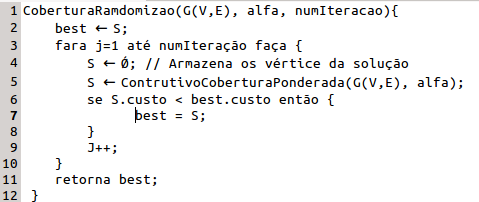
\includegraphics[scale=0.8]{rand.png}
% 		\caption{Algoritmo Flody-Warshall, a primeira matriz sem a execução do algoritmo, a segunda e resuldado do algoritmo e a terceira represeta o menor caminho do vértice v para cada vértice u}
		\label{fig:randomico}
	      \end{figure}
	      
	      \par No algoritmo Randômico é informado o grafo, um alfa entre 0.1 a 1.0 e um numero maximo de iterações.
		  Nesse algoritmo exite um best que quarda a melhor solução gerado pelo algoritmo.
		  Nas linha 5, o algoritmo Construtivo é chamado, retornando uma solu para o alfa informado.
		  Nas linhas de 6 a 8 é verificafo se a solução corrente é a melhor, caso seja, best recebe a solução.
		  
		  
	    \item Algoritmo Construtivo Randômico Reativo:
		  \par Concite em escolher o melhor canditato entre os x melhores candidatos de uma lista L de canditato previamente ordenada.
		       Onde o tamnha de x é dado pelo tamanha da L * alfa, onde 0 > alfa < 1. 
		       A cada iteração o tamanho de x é alterado escolhendo um novo alfa dentro de um array de alfas.
		       O criterio de escolha do alfa, é dado pela probabilidade do alfa, que é calculada a cada iteração.
		  \par O calculo da probabilidade de cada alfa é ralizado da seguinte forma.
		    \begin{equation}
			P[i] = \frac{Q[i]} {somaQ}			
		    \end{equation}
		    Onde Q[i] é o valor quatitativo do alfa[i].
		    \begin{equation}
		     somaQ = {\sum_{n=i}^{n} Q[i]} 
		    \end{equation}
		    Soma de todos os valores quantitativo dos alfas.		    
		    \begin{equation}
		      Q[i] = \frac{best}{M[i]}
		    \end{equation}
		    Onde best é o custo da melhor solução encontrada com o alfa[i].		    
		  
		    \newpage
		    
		    \begin{equation}
		      M[i] = \frac {C[i]}{c[i]}
		    \end{equation}		    
		    Onde M[i] é a media, C[i] é a soma de todos os custo das soluções do alfa[i] e c[i] a quatidade de vezer que o alfa[i] foi utilizado.		    
		    \\
			   
	      \begin{figure}[!htpb]
% 		\centering
		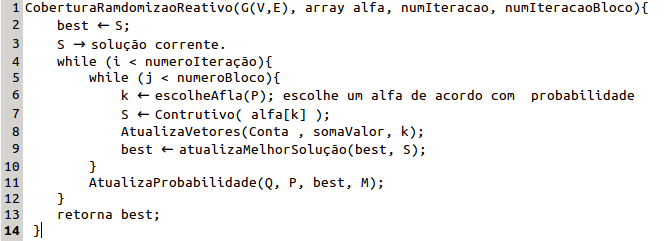
\includegraphics[scale=0.8]{reativo.png}
% 		\caption{Algoritmo Flody-Warshall, a primeira matriz sem a execução do algoritmo, a segunda e resuldado do algoritmo e a terceira represeta o menor caminho do vértice v para cada vértice u}
		\label{fig:reativo}
	      \end{figure}
	      
 	      \par O algoritmo Construtivo Randômico Reativo, recebe como parametro o grafo, uma array de alfas, um numero maximo de iterações e um numero maximo de iterações por bloco.
		   Na linha 2 e 3, são criados  a variavel "best" que armazema e melhor solução  e a variavel "S", que armazema solução corrente.
		   Na linhas 6 uma posição i é escolhida, na linha 7 o algoritmo Construtivo e armazema o resultado na variavel S, na linha 8 os vetores c e C são atualizados na posição k,
		   na linha 9 o best é atualizado com a melhor solução, na linha 11 os vetores Q, P e M são atualizados.
	      
	  \end{itemize}	  
	  
	
	\quad Funções auxiliares: 
	  \begin{itemize}
	    \item ordenaVertice: função que cria e retorna um array de vértice ordenado de forma crescente. Para ordenar é usado a função "sort" da propria linguagem.	      
	    \item decrementaGrau: decrementa o grau do vértice passado por parametro.
	    \item atualizaLista: remove o vértice passado por parametro e todos os vértice com o grau igual a 0.
	    \item melhorSolu: retorna a melhor solução entre a solução corrente e a solução atual e por referencia, retorna o custo da solução corrente e atualiza o melhor custo.
	    \item escolheAlfa: escolhe o alfa de acordo com a sua probabilidade retornado o indece do mesmo.
	     
	  \end{itemize}

    \section{Experimentos computacionais}
      \par As funções implementadas foram desenvolvidas e testadas em um computadore com sistema operacional Linux com as seguintes especificações.
      \begin{itemize}
	  \item Processador: AMD FX 6300.
	  \item Placa de Video: GeFoce GTX960.
	  \item Menoria RAM: 12GB DDR3.
      \end{itemize}
      \par Para os teste foram utilizadas 15 instacias de tamanhas diferentes todas no formato .txt. AS instacia foram baixadas do \href{http://dimacs11.cs.princeton.edu/instances/SPG-PUCN.zip}{link}.
      Cada instacia foi rodada nos algoritomos. Todos os resuldados possuem os campos; nome da instacia, NUM-NOIS-IN -> quantidade de nos, MS -> melhor solução,
      TEMP -> tempo de execulção do algoritmo em segundos, MS -> melhor solução do algoritmo (MSG -> construtivo, MSR ->randomico, MSRE -> reativo),
      ALFA -> alfa utilizado para gerar a melhor solução, NUN-IT -> numero de iterações, NUM-NOS-S -> quantidade de nos da solução.
      
      \begin{itemize}
	\item Resuldado Algoritmo Construtivo 
	\begin{figure}[!htpb]
	    \centering
	    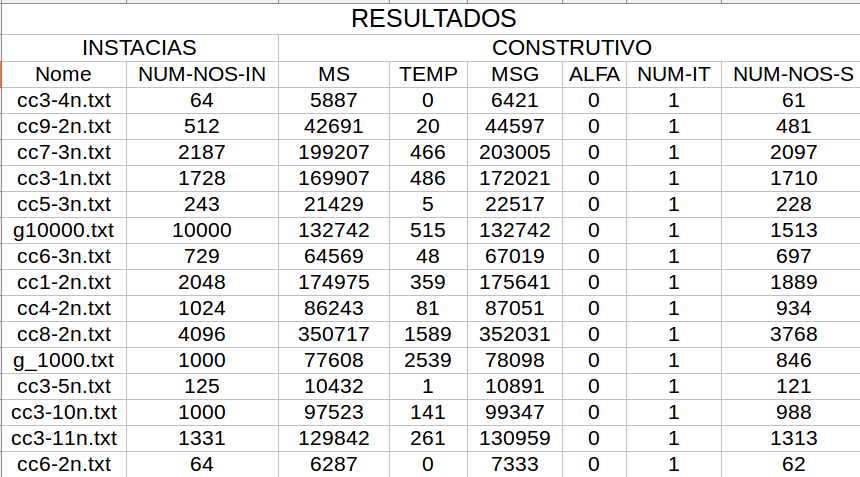
\includegraphics[scale=0.6]{resulGuloso.png}
	\end{figure} 
	 \newpage
	\item Resuldado Algoritmo Construtivo Randômico
	\begin{figure}[!htpb]
	    \centering
	    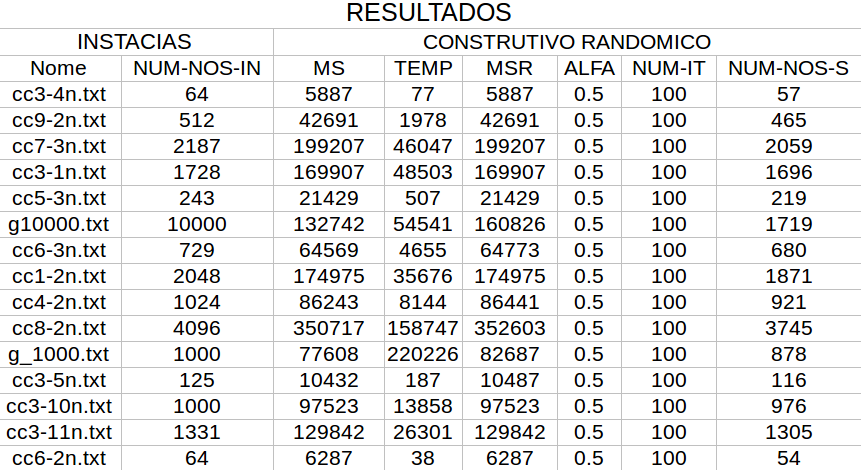
\includegraphics[scale=0.6]{resulRand.png}
	\end{figure} 
	
	\item Resuldado Algoritmo Construtivo Randômico Reativo
	\begin{figure}[!htpb]
	    \centering
	    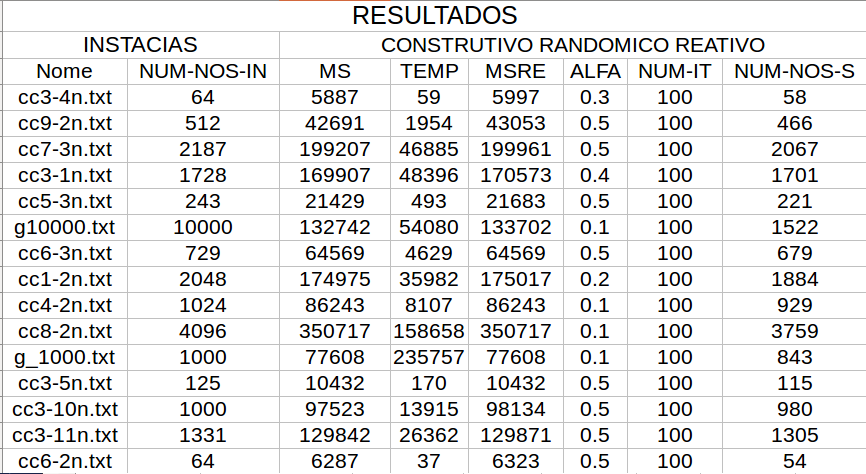
\includegraphics[scale=0.6]{resulReativo.png}
	\end{figure} 
      
      \end{itemize} 
    
    
    

\end{document} %finaliza o documento
